

\documentclass[pdflatex,sn-mathphys-num]{sn-jnl}% Math and Physical Sciences Numbered Reference Style
%%\documentclass[pdflatex,sn-mathphys-ay]{sn-jnl}% Math and Physical Sciences Author Year Reference Style
%%\documentclass[pdflatex,sn-aps]{sn-jnl}% American Physical Society (APS) Reference Style
%%\documentclass[pdflatex,sn-vancouver-num]{sn-jnl}% Vancouver Numbered Reference Style
%%\documentclass[pdflatex,sn-vancouver-ay]{sn-jnl}% Vancouver Author Year Reference Style
%%\documentclass[pdflatex,sn-apa]{sn-jnl}% APA Reference Style
%%\documentclass[pdflatex,sn-chicago]{sn-jnl}% Chicago-based Humanities Reference Style

%%%% Standard Packages
\usepackage{graphicx}%
\usepackage{multirow}%
\usepackage{amsmath,amssymb,amsfonts}%
\usepackage{amsthm}%
\usepackage{mathrsfs}%
\usepackage[title]{appendix}%
\usepackage{xcolor}%
\usepackage{textcomp}%
\usepackage{manyfoot}%
\usepackage{booktabs}%
\usepackage{algorithm}%
\usepackage{algorithmicx}%
\usepackage{algpseudocode}%
\usepackage{listings}%

% for table
\usepackage{tabularx}
\usepackage{booktabs}
\usepackage[margin=1in]{geometry}
\usepackage{array}
%%%%


\theoremstyle{thmstyleone}%
\newtheorem{theorem}{Theorem}%  meant for continuous numbers
%%\newtheorem{theorem}{Theorem}[section]% meant for sectionwise numbers
%% optional argument [theorem] produces theorem numbering sequence instead of independent numbers for Proposition
\newtheorem{proposition}[theorem]{Proposition}% 
%%\newtheorem{proposition}{Proposition}% to get separate numbers for theorem and proposition etc.
\theoremstyle{thmstyletwo}%
\newtheorem{example}{Example}%
\newtheorem{remark}{Remark}%
\theoremstyle{thmstylethree}%
\newtheorem{definition}{Definition}%
\raggedbottom
%%\unnumbered% uncomment this for unnumbered level heads

\begin{document}

\title[Exploring the Full Potential of Hyperspectral Data for Ecosystem Monitoring]{Exploring the Full Potential of Hyperspectral Data for Ecosystem Monitoring}

%%=============================================================%%
%% GivenName	-> \fnm{Joergen W.}
%% Particle	-> \spfx{van der} -> surname prefix
%% FamilyName	-> \sur{Ploeg}
%% Suffix	-> \sfx{IV}
%% \author*[1,2]{\fnm{Joergen W.} \spfx{van der} \sur{Ploeg} 
%%  \sfx{IV}}\email{iauthor@gmail.com}
%%=============================================================%%

%\author*[1,2]{\fnm{First} \sur{Author}}\email{iauthor@gmail.com}

%\author[2,3]{\fnm{Second} \sur{Author}}\email{iiauthor@gmail.com}
%\equalcont{These authors contributed equally to this work.}

%\author[1,2]{\fnm{Third} \sur{Author}}\email{iiiauthor@gmail.com}
%\equalcont{These authors contributed equally to this work.}

%\affil*[1]{\orgdiv{Department}, \orgname{Organization}, \orgaddress{\street{Street}, \city{City}, \postcode{100190}, \state{State}, \country{Country}}}

%\affil[2]{\orgdiv{Department}, \orgname{Organization}, \orgaddress{\street{Street}, \city{City}, \postcode{10587}, \state{State}, \country{Country}}}

%\affil[3]{\orgdiv{Department}, \orgname{Organization}, \orgaddress{\street{Street}, \city{City}, \postcode{610101}, \state{State}, \country{Country}}}

\abstract{Monitoring ecosystems from local to global scales is essential for understanding and managing biodiversity, biogeochemical cycles, and ecosystem services. Monitoring via \textit{in situ} methods provides important details but with limited spatial coverage, generally not suitable for capturing large-scale ecosystem states and changes. Hyperspectral and multispectral remote sensing, ideally combined with machine learning integrating data from \textit{in situ} measurements, provide a powerful approach to support ecological monitoring by enabling continuous and scalable observations of plant traits and ecosystem dynamics. This perspective paper explores the integration of hyperspectral and multispectral remote sensing with machine learning for enhanced ecological monitoring. We discuss the potential of these technologies to improve the quantification of plant traits, support global ecosystem monitoring, and quantify vegetation resistance, resilience, and responses to environmental stress; as well as key challenges including data availability, computational constraints, and interdisciplinary collaboration. Opportunities to overcome these barriers through advanced data fusion, open science, and international cooperation are presented. By proposing practical approaches that address both the potential and challenges of using multi- and hyperspectral data for ecosystem monitoring, this work aims to engage both the remote sensing and ecology communities.}

%\abstract{
%Accelerating climate change and increasing climate extremes are altering ecosystem functioning worldwide, yet our capacity to monitor vegetation responses remains largely based on broadband spectral indices that provide limited physiological insight. Understanding how ecosystems resist, respond to, and recover from climatic disturbances requires observations that directly reflect plant functional processes.

%Plant functional traits such as leaf pigments, nitrogen concentration, structural properties, and water-related traits quantify the biochemical and physiological states that regulate carbon uptake, transpiration, and stress tolerance. Hyperspectral remote sensing enables the retrieval of multiple traits with physiological interpretability, but its limited temporal continuity constrains its application for long-term climate analyses. We propose establishing temporally resolved plant trait time series by integrating hyperspectral-derived trait products with dense multispectral archives, allowing hyperspectral information to be extended across time without reconstructing full spectral signals.

%Trait time series provide a process-informed observational framework for quantifying ecosystem resistance, recovery trajectories, and legacy effects under climate extremes. By linking satellite observations more directly to plant physiological states, trait-based monitoring offers new opportunities to constrain ecosystem and carbon cycle models and to assess climate-ecosystem feedbacks across scales. Positioning plant traits as a central observational variable can strengthen the mechanistic understanding of ecosystem dynamics in a rapidly changing climate.

%}


\keywords{Hyperspectral, multispectral, imaging spectroscopy, remote sensing, machine learning, plant traits, genetic diversity, climate change, extreme weather, vegetation resilience, ecosystem functioning}
\maketitle

\section{Main}\label{sec1}



% General Introduction
Functional ecosystems are the foundation of planetary health and human well-being \cite{ipbes2019,hernandez2022ecosystem}. They incorporate the maintenance and stabilisation of key Earth system processes, providing the resources and habitat for life on Earth \cite{ipcc2022wg2ch2}. The accelerating pace of human-induced climate change and intensification of land use places stress on ecosystems worldwide, negatively impacting their functioning. Plants, particularly trees in forest ecosystems, are critical components of the terrestrial carbon cycle, storing approximately 80\% of terrestrial carbon as biomass and thereby playing a central role in global climate regulation \cite{pan2011large} in addition to being among Earth's main primary producers of energy for all other branches on the tree of life. They must adapt not only to the average changes in the Earth's climate, but also to its increased variability, bringing greater risks of extreme weather events such as prolonged droughts, heatwaves, late frosts, storms and floods \cite{lindner2010climate,seidl2017}. Detailed and continuous monitoring is crucial for understanding ecosystem responses to environmental changes and supporting effective conservation, restoration, and management strategies \cite{mahecha2024biodiversity}.

% traits
Plant functional traits provide a mechanistic description of how vegetation regulates carbon, water, and energy exchange with the atmosphere. Traits such as leaf chlorophyll content, nitrogen concentration, leaf mass per area (LMA), leaf area index (LAI), and equivalent water thickness (EWT) quantify biochemical composition, physiological capacity, and structural properties of plants. Unlike broadband spectral indices, these traits correspond directly to physiological processes including photosynthesis, transpiration, nutrient limitation, and stress tolerance. Because traits link plant physiology to ecosystem functioning and climate feedbacks, they represent a consistent state variable that can bridge field measurements, remote sensing observations, and ecosystem models. Monitoring ecosystems through temporally resolved trait dynamics therefore enables the assessment of vegetation condition, resistance to disturbances, and recovery processes in a process-oriented framework rather than through indirect spectral proxies.

In this perspective, we argue that constructing temporally consistent plant trait data cubes should become a central objective of ecosystem monitoring. Hyperspectral remote sensing enables the retrieval of multiple plant traits with physiological interpretability, but current spaceborne hyperspectral observations lack dense temporal coverage. We therefore discuss how hyperspectral-derived traits can be combined with temporally frequent multispectral observations to build consistent trait time series, and how such data products can transform ecosystem science. A non-exhaustive overview of retrievable plant traits and their ecological relevance is summarised in Table \ref{tab1}.

% Limitations of Traditional Monitoring Methods
\textit{In situ} observations are the backbone of ecosystem monitoring at local scales, whereas global initiatives additionally rely on remote sensing data \cite{balsamo2018satellite}. \textit{In situ} ecological monitoring is typically precise and essential for improved process understanding. However, such local approaches are constrained by several limitations. \textit{In situ} ecosystem monitoring either relies on manual data collection, including plot-based investigations, e.g. of plant traits, species sampling, or on very specialised long-term environmental parameter measurements, such as land-atmosphere fluxes of CO$_2$, e.g. in ecological monitoring networks. These intensive measurements are time- and cost-intensive and thus only applied to specific sites. Consequently, \textit{in situ} networks, such as ForestGEO \cite{anderson2015ctfs} and ILTER \cite{mirtl2018genesis}, attempt to expand long-term, site-based ecological monitoring, but remain limited in spatial extent due to logistical scalability\cite{magurran2010long}. In fact, such data that are indispensable for improved process understanding, are typically affected by spatial sampling biases \cite{verheyen2012driving, mahecha2017detecting} and fail to capture processes in spatially continuous manner and may miss changes in ecosystem structure, function, and disturbance regimes, especially in remote or inaccessible regions. %Moreover, data collection involves a trade-off between being labour-intensive and costly versus achieving extensive temporal coverage and high revisit frequency \cite{magurran2010long}. 

An alternative avenue is citizen science approaches. In fact, over the last years we observed substantial advancements. Flagship initiatives such as iNaturalist, GBIF, eBird, and iTree have expanded public engagement and species observation efforts. However, despite their effort, these data cannot compensate for the existing gaps, which are typically much noisier than academic collections \cite{bonney2021expanding,schiller2021deep}.
%% Additionally, global databases such as sPlotOpen \cite{sabatini2021splotopen} and TRY \cite{kattge2020try} aggregate plot-based vegetation composition and plant trait data, enabling broad-scale ecological analyses.  In parallel, citizen science platforms—including iNaturalist, GBIF, eBird, and iTree—have expanded public engagement and species observation efforts \cite{bonney2021expanding}. However, despite substantial advances across these complementary approaches, none fully overcome the limitations of spatial coverage, revisit frequency\cite{magurran2010long}, and standardisation\cite{schiller2021deep}.

% The Advent of Multispectral Remote Sensing
Satellite remote sensing, particularly multispectral remote sensing, has transformed ecosystem observation and assessment, particularly for understanding the contribution of plants \cite{andrew2014potential,pettorelli2018satellite}. 
Open data products offer verifiable means of deriving complete spatial coverage of environmental information for large areas at different spatial and temporal resolutions in a consistent manner. Multispectral remote sensing has thus been widely used in forest ecosystem monitoring, including vegetation coverage assessment, vegetation health evaluation \cite{zarco2019chlorophyll,brown2025grounded,cherif2022deepforest}, the tracking of vegetation phenology \cite{dronova2022remote}. However, with a few exceptions, remote sensing data rarely provide information in physical units directly corresponding to those of \textit{in situ} vegetation measurements: reflectance data must be translated into properties of interest. Remote sensing data thus essentially always require combination with \textit{in situ} data to support their interpretation, either established via empirical relations, machine learning methods, or models, e.g. process-based radiative transfer models. Once interpretation is achieved, remote sensing becomes much more essential for understanding ecosystems across scales \cite{cavender2025spectral}. 
In addition to the need for informative \textit{in situ} data, there are other challenges to the gainful interpretation of remote sensing data from multispectral sensors. In forest ecosystems, optical remote sensing observation typically captures only the upper canopy, leaving sub-canopy and understory vegetation and their condition largely unobserved. Data availability for multispectral and other optical sensors may be restricted by cloud cover, particularly during wet seasons. Land-use practices, such as mowing, prescribed burning, grazing, and thinning, additionally alter the interpretation of remote sensing signals. Furthermore, variations in sensor design and the evolution of sensors over time can introduce inconsistencies in data availability and interoperability. Finally, the spatial resolution of imagery dictates the appropriate mapping scale, and no single resolution is universally optimal for all ecosystem applications.

%hyperspectral data
Hyperspectral remote sensing has been developed over the past decades, providing continuous and narrow spectral bands in contrast to the wider, discontinuous, and discrete bands provided by multispectral sensors. These hyperspectral bands improve and enable the retrieval of plant trait information across biochemistry (e.g. pigments and water content), physiological process (parameters such as light use efficiency - LUE), and structure (parameters such as leaf area index - LAI, leaf inclination) (see Fig.~\ref{fig1} and Table~\ref{table1}. Such biochemical leaf and canopy trait information is highly related to carbon fixation and sequestration \cite{richardson2002evaluation,le2004towards,blackburn2007hyperspectral}. Although hyperspectral remote sensing has proven powerful, existing high-quality hyperspectral data have been limited for a long time to airborne acquisitions with restricted spatial and temporal coverage, confining its use to local or regional case studies and hindering regional to global monitoring.

%However, current high-quality airborne hyperspectral data acquisitions are limited in their spatiotemporal coverage, and spaceborne hyperspectral missions are newer and generally have lower signal-to-noise ratios compared to multispectral data due to the limited photon density per band. 

\begin{figure}[h]
\centering
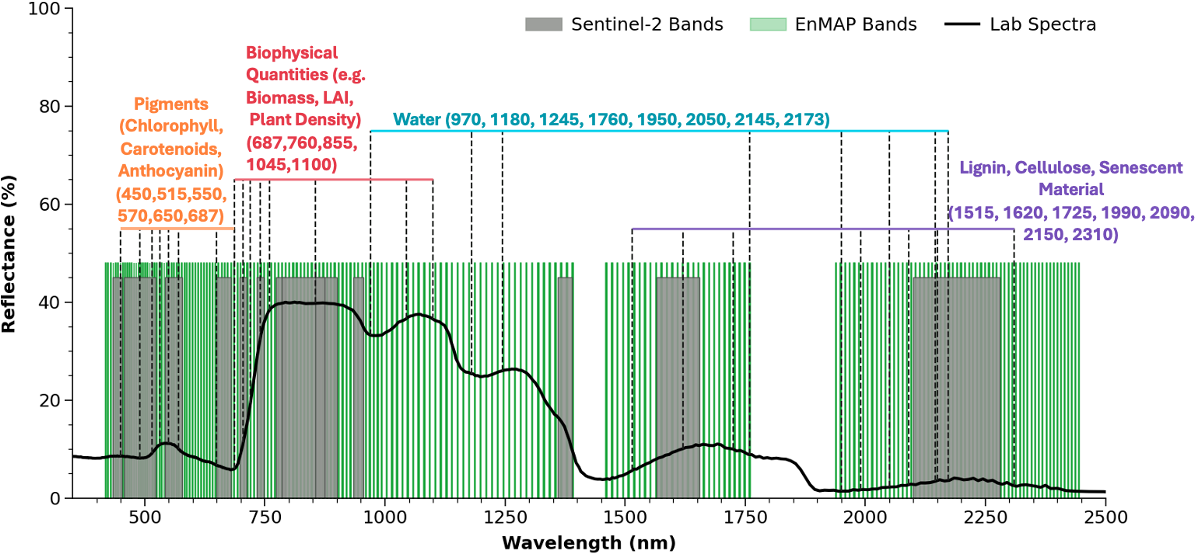
\includegraphics[width=1\textwidth]{figures/fig1_v6.png}
\caption{Vegetation spectra acquired from a laboratory spectrometer alongside the spectral bands of a multispectral sensor (Sentinel-2) and hyperspectral sensor (EnMAP) used in remote sensing. To improve readability, EnMAP spectral band widths are reduced to one twentieth of their actual size to minimise overlap. Highlighted are spectral domains sensitive to specific vegetation variables, with absorption features adapted from \citet{thenkabail2013selection,hank2019spaceborne}. }
\label{fig1}
\end{figure}


\renewcommand{\tabularxcolumn}[1]{>{\raggedright\arraybackslash}p{#1}}
\small
\begin{table}[htbp]
\begin{tabularx}{\textwidth}{
  p{\dimexpr 0.15\textwidth}  % Trait Description
  p{\dimexpr 0.25\textwidth}  % Relevant Process
  p{\dimexpr 0.40\textwidth}  % Ecosystem Process
  p{\dimexpr 0.05\textwidth}  % Retrieval Source
}
\toprule
\textbf{Trait (Abbreviation)} & \textbf{Physiological Process} & \textbf{Ecosystem Process / Climate Relevance} & \textbf{Retrieval Source} \\
\midrule
Chlorophyll content (Chl) & Photosynthesis & Strong proxy for photosynthetic capacity, productivity, and nutrient stress detection. & HS; MS\\
\midrule
Carotenoid content (Car) & Photoprotection, light harvesting & Indicates photoprotection, useful for tracking drought or high-light stress. & HS; MS\\
\midrule
Anthocyanin content (Anth) & Stress response, Ultraviolet (UV) protection & Sensitive to abiotic stress (UV, cold), less directly linked to productivity. & HS; MS \\
\midrule
Nitrogen content (N) & Protein synthesis, photosynthesis & Controls photosynthesis, growth, and is an early indicator of nutrient limitation. & HS\\
\midrule
Phosphorus content (P) & adenosine triphosphate (ATP) synthesis, nucleic acids & Limits productivity especially in tropical or weathered soils; links to C allocation strategies. & HS\\
\midrule
Potassium content (K) & Osmoregulation, stomatal conductance & Key to osmotic regulation and drought tolerance; affects stomatal conductance. & HS\\
\midrule
Magnesium content (Mg) & Chlorophyll core, enzyme activation & Central to chlorophyll molecule and enzyme function; affects stress sensitivity. & HS\\
\midrule
Sulfur content (S) & Amino acids, redox balance & Indirectly affects protein synthesis and redox regulation; harder to monitor. & HS\\
\midrule
Boron content (B) & Cell wall structure, reproductive development & Important for reproduction and cell wall function; indirect ecosystem effects. & HS\\
\midrule
Copper content (Cu) & Electron transport, redox reactions & Involved in redox reactions, minor influence at ecosystem scale. & HS\\
\midrule
Manganese content (Mn) & Photosystem II activity, redox regulation & Important in photosynthesis and Reactive Oxygen Species (ROS) control, but limited large-scale impact. & HS\\
\midrule
Carbon content (C) & Biomass accumulation, respiration & Key trait in leaf economic spectrum; predicts trade-offs in resource use and longevity. & HS \\
\midrule
Calcium content (Ca) & Cell wall stability, signalling, & Used in biomass and stoichiometric modelling; influences decomposition. & HS\\
\midrule
Cellulose content & Cell wall formation, structural support & Structural role in cell walls; not often modelled in ecosystem responses. & HS \\
\midrule
Fibre content & Mechanical support, digestion resistance & Strong predictor of litter decomposition rates and carbon turnover. & HS\\
\midrule
Lignin content & Cell wall rigidity, decomposition resistance & Key to biomass structure and carbon cycling via decomposition. & HS\\
\midrule
Leaf Mass per Area (LMA) & Photosynthetic efficiency, leaf economics & Influences herbivory and digestibility, affects trophic interactions. & HS; MS\\
\midrule
Leaf Area Index (LAI) & Radiation interception, productivity & Directly linked to canopy photosynthesis, water use, and light interception. & HS; MS\\
\midrule
Equivalent Water Thickness (EWT) & Leaf hydration, transpiration & Reflects drought sensitivity, transpiration regulation, and water availability. & HS; MS \\
\midrule
Non-Structural Carbohydrates content (NSC) & Growth, respiration, recovery & Strong predictor of stress resilience, recovery from disturbance, and survival. & HS\\
\bottomrule
\end{tabularx}
\caption{Plant traits can be estimated from hyperspectral (HS) and/or multispectral (MS) data. Their relevance to physiological and ecosystem processes, as well as their remote sensing retrieval sources, are summarised in the following traits list, adapted from the hyperspectral trait retrieval study by Cherif et al. \cite{cherif2023spectra}.}
\label{table1}
\end{table}


% missions
Recent advancements, however, are addressing these limitations and shifting the paradigm. New spaceborne hyperspectral missions, such as\cite{alonso2019data}, GaoFen-5 (2018)\cite{liu2019advanced}, HISUI (2019)\cite{iwasaki2011hyperspectral}, PRISMA (2019)\cite{loizzo2019prisma}, EnMAP (2022)\cite{guanter2015enmap}, EMIT (2022), have gradually enabled high-quality global hyperspectral data collection. Key upcoming operational missions are scheduled for launch, including CHIME A (2028) and CHIME B (2030) \cite{nieke2018towards}, the SBG mission\cite{cawse2021nasa}, set for 2028, and under-development SHALOM\cite{feingersh2015shalom}. These missions will significantly improve spatial coverage and revisit times, enabling a more detailed and frequent global hyperspectral archive, given that an intercalibration of these sensors is achieved. %, because hyperspectral sensors generally have lower signal-to-noise ratios compared to multispectral data due to the limited photon density per band. 
 

% research gap
Hyperspectral data thus promise great opportunities for quantifying plant traits with upcoming spaceborne missions. However, key challenges remain in realising this potential for effective ecosystem monitoring in concert with established techniques.
First, long-term ecosystem monitoring requires consistent historical data spanning decades, which hyperspectral observations currently lack. While new missions are underway, the absence of historical coverage presents a challenge for long-term ecosystem analyses. Therefore, a strategic approach is needed to bridge this gap and enable comprehensive monitoring over time.
Second, assuming this gap is addressed, it has not yet been determined how hyperspectral data can be integrated into existing long-term regional and global monitoring frameworks to maximise its potential and enhance analytical capacity and ecological insight.
This paper tackles the first challenge in Section \ref{sec2} and explores the second in Section \ref{sec3}, offering a path forward for leveraging hyperspectral data in ecosystem monitoring.


\section{Building consistent time series with hyperspectral information} \label{sec2}

Long-term ecosystem monitoring requires temporally consistent observations of plant functional traits. While hyperspectral remote sensing enables the retrieval of multiple physiologically meaningful traits, current spaceborne hyperspectral missions provide sparse temporal coverage and relatively low revisit frequency. This limitation restricts the direct construction of dense trait time series needed to analyse phenology, stress dynamics, and recovery processes. To overcome this constraint, we propose using temporally frequent multispectral observations to extend hyperspectral-derived trait information. By leveraging time periods where hyperspectral and multispectral data overlap, models can be trained to predict hyperspectral-derived traits from multispectral time series, thereby constructing temporally dense trait data cubes.


%The benefits of the rich spectral information of hyperspectral data are currently affected by their limited temporal resolution, as the technology is relatively new. The current lack of dense time series has restricted their integration into ecosystem studies, which demand continuous or frequent observations to monitor dynamic processes such as phenology, stress responses, or productivity. The scarcity of temporally dense spaceborne hyperspectral data stems from short historical archives and low revisit frequencies of current hyperspectral sensors. Even when some hyperspectral acquisitions are available, the number of time points is typically too sparse for constructing robust time series needed in ecological analyses \cite{lausch2015deriving}. To address this, we propose using multispectral data with high temporal frequency, such as those from Sentinel-2, to extend the temporal coverage of hyperspectral-derived information. By correlating hyperspectral and multispectral observations at overlapping time points, models can be trained to predict hyperspectral-derived plant traits across more timesteps using multispectral data (see Fig.~\ref{fig2}). 

\begin{figure}[h]
\centering
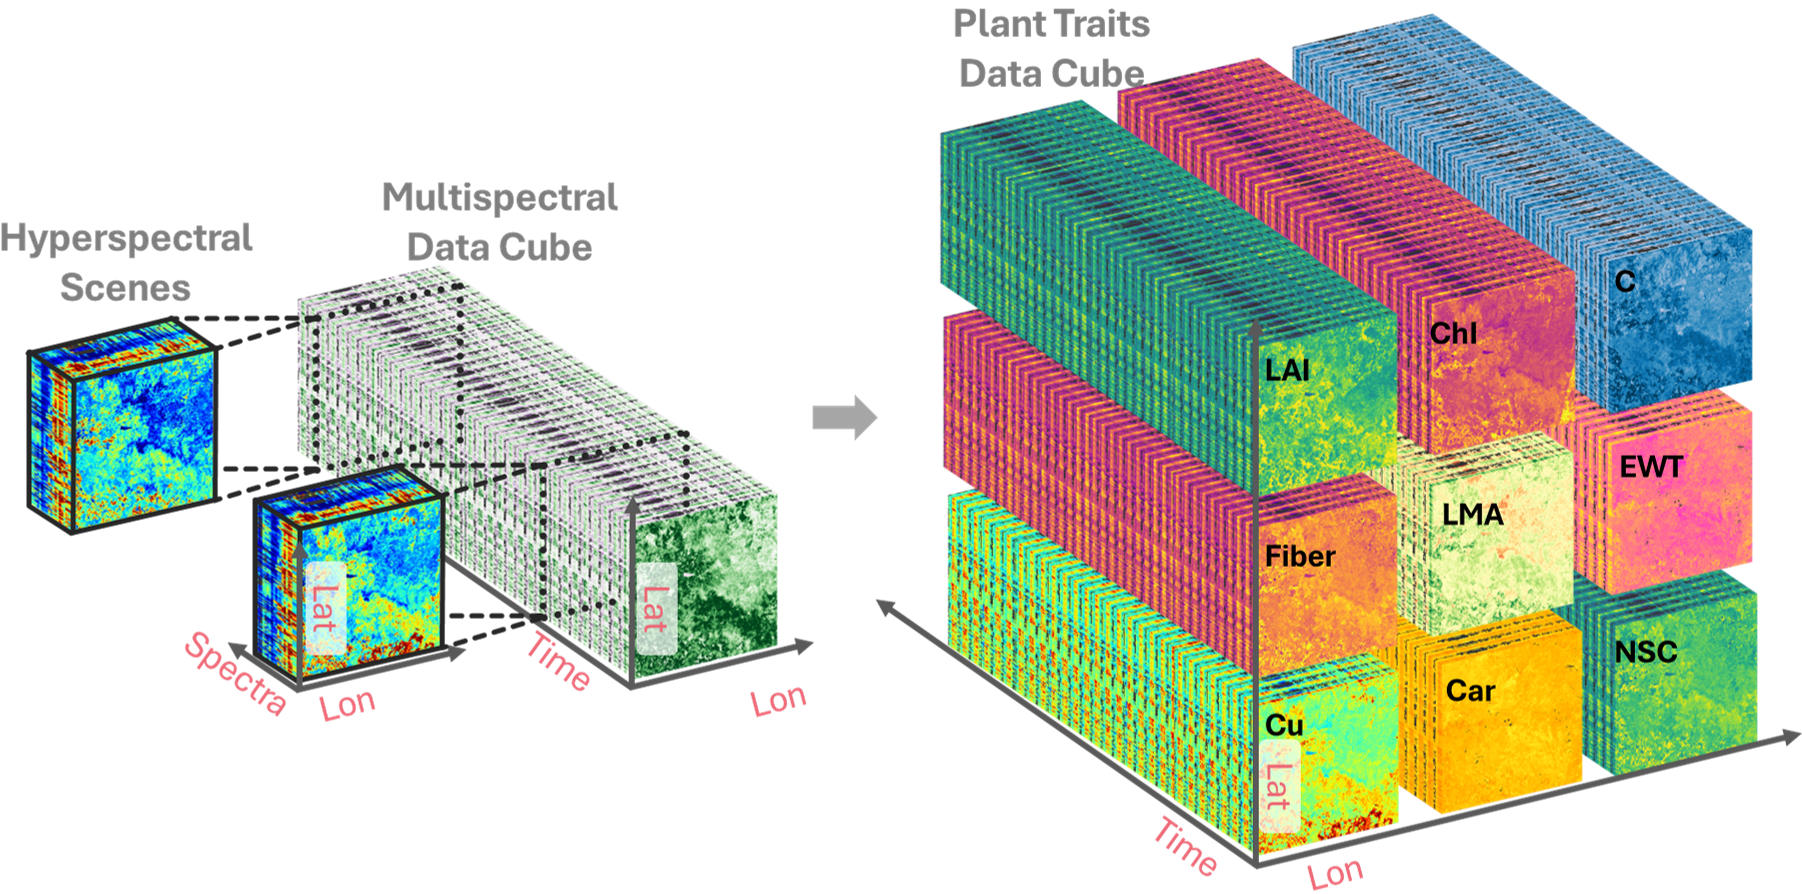
\includegraphics[width=0.85\textwidth]{figures/fig2_v6.png}
\caption{Conceptual illustration of constructing a time series using hyperspectral and multispectral data. On the left, several hyperspectral data cubes (EnMAP; spatial and spectral dimensions) and a time series multispectral data cube (Sentinel-2; spatial and temporal dimensions) are shown. Spectral bands of Sentinel-2 are omitted for clarity. The multispectral data provide a dense temporal baseline, while the hyperspectral data, available at fewer time points, are fused with the multispectral observations. On the right, the resulting plant trait data cube, derived from hyperspectral bands, benefits from the dense and stable temporal coverage provided by the multispectral time series. The demonstration area is the Bavarian Forest National Park. The data cube is visualised using Lexcube \cite{sochting2023lexcube}.}
\label{fig2}
\end{figure}


To avoid the computational and data management burden of modelling hundreds of spectral bands across time, we recommend using hyperspectral observations to first retrieve key plant traits (e.g., chlorophyll content, leaf area index, leaf dry matter) \cite{cherif2023spectra}. These traits can then be modelled over time using multispectral time series data, significantly reducing data dimensionality and enhancing ecological interpretability.

% uncertainty control
Retrieving plant traits from hyperspectral data typically involves spectral preprocessing and correction (e.g., atmospheric correction, noise filtering) and model-based trait estimation. Trait estimation is commonly implemented using statistical regressions (e.g., PLSR), physical model inversion (e.g., PROSAIL), or machine learning approaches (e.g., random forest, CNNs) trained on reference trait datasets \citep{Blackburn2007, LeMaire2004, Cherif2023}. Model calibration relies on trait reference data collected from \textit{in situ} or laboratory measurements (e.g., leaf chlorophyll content, LMA, nitrogen). To ensure generalizability, calibration is ideally conducted using a representative, diverse training dataset covering the range of canopy structures, species, and environmental conditions relevant to the study area \citep{Verrelst2015, Kattenborn2019}. Validation of hyperspectral-derived traits is typically done using an independent set of trait observations not included in the calibration. Statistical metrics such as R$^2$, RMSE, and bias are used to assess model performance. When repeated \textit{in situ} or laboratory data are not available, cross-validation or transfer learning methods may be used to estimate uncertainty across space or time. Major sources of uncertainty include sensor noise, variability in viewing geometry, imperfect atmospheric correction, and mismatch in spatial scale between hyperspectral imagery and field plots \citep{Schweiger2020, Mederer2025}. To mitigate these uncertainties, recent work has explored hybrid models that combine radiative transfer simulations with empirical machine learning, or use physics-informed neural networks to constrain trait predictions with ecological realism \citep{Sun2024, She2024}. As a best practice, we recommend reporting uncertainty estimates (e.g., prediction intervals, ensemble spread) alongside trait predictions and validating results across multiple sites and time periods where possible.

The temporal construction between hyperspectral or hyperspectra-estimated images and multispectral data are relatively new, but in the past two decades, remote sensing and computer vision researchers have developed numerous methods for fusing hyperspectral and multispectral data, primarily to improve the spatial resolution \cite{yokoya2017hyperspectral} of hyperspectral images. These spatial fusion models aim to reconstruct high-spatial-resolution hyperspectral data by exploiting the spectral redundancy between multispectral and hyperspectral imagery. Many of the models, designed initially for spatial fusion, such as sparse representation-based methods, deep learning fusion networks, or hybrid regression frameworks, can be repurposed to enhance temporal resolution. These models are fundamentally based on learning the relationships between multispectral and hyperspectral spectral patterns, and this principle can be extended to temporal interpolation. The survey of these methods, though not exhaustive here, can be grouped into four main categories. Model-based approaches include traditional dimensionality reduction techniques (e.g., Intensity-Hue-Saturation (IHS) transformation, Principal Component Analysis (PCA)), multiresolution analysis methods (e.g., wavelet, contourlet), and subspace-based models such as Coupled Nonnegative Matrix Factorization (CNMF) \cite{yokoya2017hyperspectral}. Sparse representation-based methods encompass joint sparse representation, convolutional sparse coding, and spatial-spectral sparse representation techniques \cite{xing2022fusion,dian2019multispectral}. Deep learning-based approaches cover a broad spectrum of architectures, including Convolutional Neural Networks (CNNs), autoencoders, Generative Adversarial Networks (GANs), transformers, hybrid CNN-transformer models, and attention-enhanced frameworks \cite{khader2022model,gao2023enhanced,jia2023multiscale,hong2021interpretable}. These methods can be used to correlate hyperspectral and multispectral data and leverage multispectral observations to estimate missing hyperspectral information at unobserved timesteps within the same study area. However, reconstructing the full hyperspectral signal as an intermediate step prior to plant trait estimation can be computationally inefficient and prone to compounded uncertainty, first during spectral reconstruction, and then again during trait estimation from the reconstructed hyperspectral signal. An alternative strategy would consist of first reconstructing pseudo-hyperspectral imagery from multispectral observations and subsequently retrieving plant traits from the reconstructed spectra. While such an approach may benefit from higher spatial coverage, it introduces compounded uncertainty, as errors from spectral reconstruction propagate into trait estimation. Directly modelling trait dynamics from multispectral time series using hyperspectral-derived trait products as training targets reduces dimensionality and avoids intermediate spectral reconstruction. For ecosystem applications, we therefore consider trait-level modelling the more parsimonious and ecologically interpretable pathway.



To overcome these limitations, multi-modal models can bypass spectral reconstruction by learning task-relevant representations directly from different sources (also known as different modalities). Among these models, transformer-based architectures have shown promise for handling pixel-level time series from multi-modal data. From here, there are two pathways to follow: a classical supervised approach with annotated data, or a self-supervised approach to pre-train the model with unlabelled data. While the first case is straightforward, collecting the required data can be expensive, and availability is limited, delivering overfitted models due to the few samples used in training. In the second case, while there is no need for labelled data, the resources needed to pretrain a model on a large dataset that is able to capture an accurate representation of Earth processes can be enormous. However, the second case brings the opportunity to fine-tune the model for different downstream tasks, such as crop type classification, land cover mapping, or algal bloom prediction. One illustrative example is the Pretrained Remote Sensing Transformer (Presto) \cite{tseng2023lightweight}, which aligns closely with our proposed approach of using temporally dense multi-spectral data. Presto learns temporal representations from multi-modal time series data (e.g., Sentinel-1, Sentinel-2), combined with auxiliary metadata such as topography and climate variables. It employs a masked autoencoding strategy to learn informative temporal embeddings by reconstructing missing spectral bands or timesteps. Although this approach has not yet been applied to plant trait prediction, its architecture is well-suited for this purpose. Moreover, the framework can be extended to flexibly accommodate hyperspectral data by enabling the model to ingest a broader and variable number of spectral bands, so that when hyperspectral observations are available, they can directly enrich the input representation and improve trait prediction.

% validation
For temporal validation, we recommend cross-year or leave-one-period-out validation schemes, in which hyperspectral acquisitions from selected years are excluded during training and used to evaluate backcasted trait predictions derived from multispectral data. Where early hyperspectral observations are available, they can serve as independent benchmarks for assessing the reliability of trait backcasting across time.


% one paragraph with data cube technique

\section{What trait time series enables for ecosystem science} \label{sec3}

Trait data cubes derived from the fusion of hyperspectral and multispectral observations fundamentally change the type of ecological variables that can be monitored consistently in space and time. Rather than relying on broadband proxies of canopy greenness or structure, these data products provide temporally resolved, physiologically interpretable descriptors of vegetation state and function. This shift from spectral indices to trait-based observables represents a qualitative change in ecological inference from space, with consequences for how ecosystem condition, stress responses, and recovery processes can be analysed across scales.

\subsection{Trait-based vegetation condition and stress dynamics}

Broadband spectral indices such as NDVI or EVI have long been used to track vegetation dynamics \cite{zeng2022optical}, but their ecological interpretability is inherently limited. These indices integrate signals from multiple biophysical and structural components and often respond similarly to distinct stressors. As a result, comparable index trajectories can arise from fundamentally different physiological pathways, such as water limitation, nutrient stress, thermal damage, or phenological transitions. This ambiguity becomes particularly problematic under climate extremes, when multiple stress processes may co-occur or unfold sequentially.

Trait time series provide a more detailed observational basis. Hyperspectral-derived traits, including pigments, water-related traits, and structural or defensive properties, correspond more directly to plant physiological processes that regulate photosynthesis, transpiration, plant water status, and stress tolerance. When tracked over time, these traits describe vegetation condition in terms of functional states rather than spectral proxies, including changes associated with phenological transitions. Importantly, combinations of trait dynamics can reveal distinct stress syndromes, reflecting different underlying physiological constraints, that are not separable using greenness-based indices alone.

This trait-based perspective enables an event-oriented analysis of ecosystem responses. During and after extreme events such as droughts or heatwaves, trait dynamics allow the consistent quantification of resistance (the magnitude of functional change during disturbance), recovery (the trajectory back towards pre-disturbance states), and lag or legacy effects (persistent deviations after apparent recovery). These components of ecosystem response are central to ecological theory, yet have been difficult to assess at large scales using remote sensing. Trait data cubes provide a means to estimate these quantities using variables that are mechanistically linked to plant function, enabling comparison across events, ecosystems, and climatic contexts.

While trait anomalies may in some cases precede changes in broadband indices, the primary value of trait-based monitoring lies not in earlier detection alone, but in improved attribution. Trait dynamics support the identification of which physiological constraints are changing. This distinction is essential for interpreting ecosystem responses under increasing climate variability and for moving beyond descriptive monitoring towards process-informed analysis.

\subsection{Ecological implications across temporal and spatial scales}

The availability of temporally explicit trait data cubes has implications beyond the analysis of individual stress events. At the level of communities, trait time series provide access to dynamic trait distributions rather than static mean values. Temporal variability in traits reflects shifts in functional composition, intraspecific variability, and differential responses among co-occurring species. As such, trait dynamics offer a functional bridge between individual physiological responses and community-level properties related to stability, resilience, and adaptive capacity. Remotely sensed trait variability thus complements field-based trait ecology by extending functional perspectives across space and time.

At ecosystem and modelling scales, trait data cubes offer a new class of empirical constraints. Many ecosystem and carbon cycle models rely on static trait parameterisations or categorical plant functional types, limiting their ability to represent transient stress responses and recovery processes. Temporally resolved traits promisingly provide observation-based information on changing physiological states that can be used to evaluate, constrain, or benchmark model behaviour, particularly under extreme conditions. In this context, traits are not proposed as replacements for existing models, but as observable state variables that link remote sensing, field observations, and model representations more directly.

Across these scales, the key contribution of trait data cubes lies in redefining what can be observed consistently from space. By decoupling ecological variables from individual sensors and spectral indices, trait-based observables support comparative analyses across regions and time periods and align remote sensing products more closely with ecological theory. This shift enables ecologists to pose questions about ecosystem function, stress, and recovery that were previously difficult to address using large-scale observations alone.




%\section{The full ecological potential of hyperspectral data} \label{sec3}

%Once the first challenge is addressed, namely, the extension of hyperspectral-retrieved plant traits into temporal dimensions and space. This enables the construction of trait data cubes. A data cube is a multidimensional array of gridded data organised along labelled axes (e.g., space, time, variables), ideally cloud native and analysis-ready \cite{mahecha2020earth, montero2024earth}. The perspective of generating trait data cubes holds significant promise for advancing ecological analysis. Unlike traditional multispectral vegetation indices (e.g., NDVI), which provide limited physiological insights given that the signals typically encode a wide range of processes. In particular, they shall offer a functional lens to monitor vegetation states, functions, and processes with greater precision. In this section, we outline several application pathways that demonstrate the transformative potential of such data product in plant and ecosystem sciences.


%\subsection{Example 1: Vegetation Condition Assessment Beyond Classical Spectral Indices}

%Multispectral data estimated spectral indices, such as NDVI, are widely used to monitor vegetation dynamics but are sensitive not only to canopy greenness, their intended target, but also to background soil reflectance, atmospheric variability, and viewing geometry. These limitations become particularly pronounced under sparse vegetation or drought conditions, where the signal-to-noise ratio decreases and interpretability is reduced \citep{huete2002overview}. Indices derived from broadband reflectance, such as NDVI, EVI, or the tasseled cap transformation (brightness, greenness, wetness) \citep{crist1984tasseledcap}, aggregate signals from multiple biophysical sources and often fail to disentangle distinct physiological processes.

%In contrast, the hyperspectral trait cube enables the retrieval of physiologically and structurally meaningful variables—such as leaf water content (EWT), nitrogen concentration, specific leaf area (SLA), chlorophyll, and anthocyanins—that correspond more directly to plant function. These traits offer higher specificity and reduced sensitivity to confounding non-vegetation signals, making them more robust for assessing underlying drivers of vegetation change.

%Figure~\ref{fig3} illustrates a comparison between hyperspectral-derived traits and spectral indices for a forest pixel observed between 2018 and 2019. While the trait time series (left) exhibits smooth, continuous seasonal trajectories consistent with known ecological dynamics, the spectral indices (right) display abrupt jumps and discontinuities. These irregularities are partly due to data gaps and atmospheric noise in the unprocessed Sentinel-2 reflectance, but they also reflect the broader limitations of proxy-based indices. Traits derived from hyperspectral data capture distinct functional dimensions—such as water status, nutrient allocation, and photosynthetic capacity—and provide direct insight into what is changing in the system. Even when derived from temporally sparse hyperspectral observations, the trait cube delivers consistent signals and functional interpretability.

%\begin{figure}[h]
%\centering
%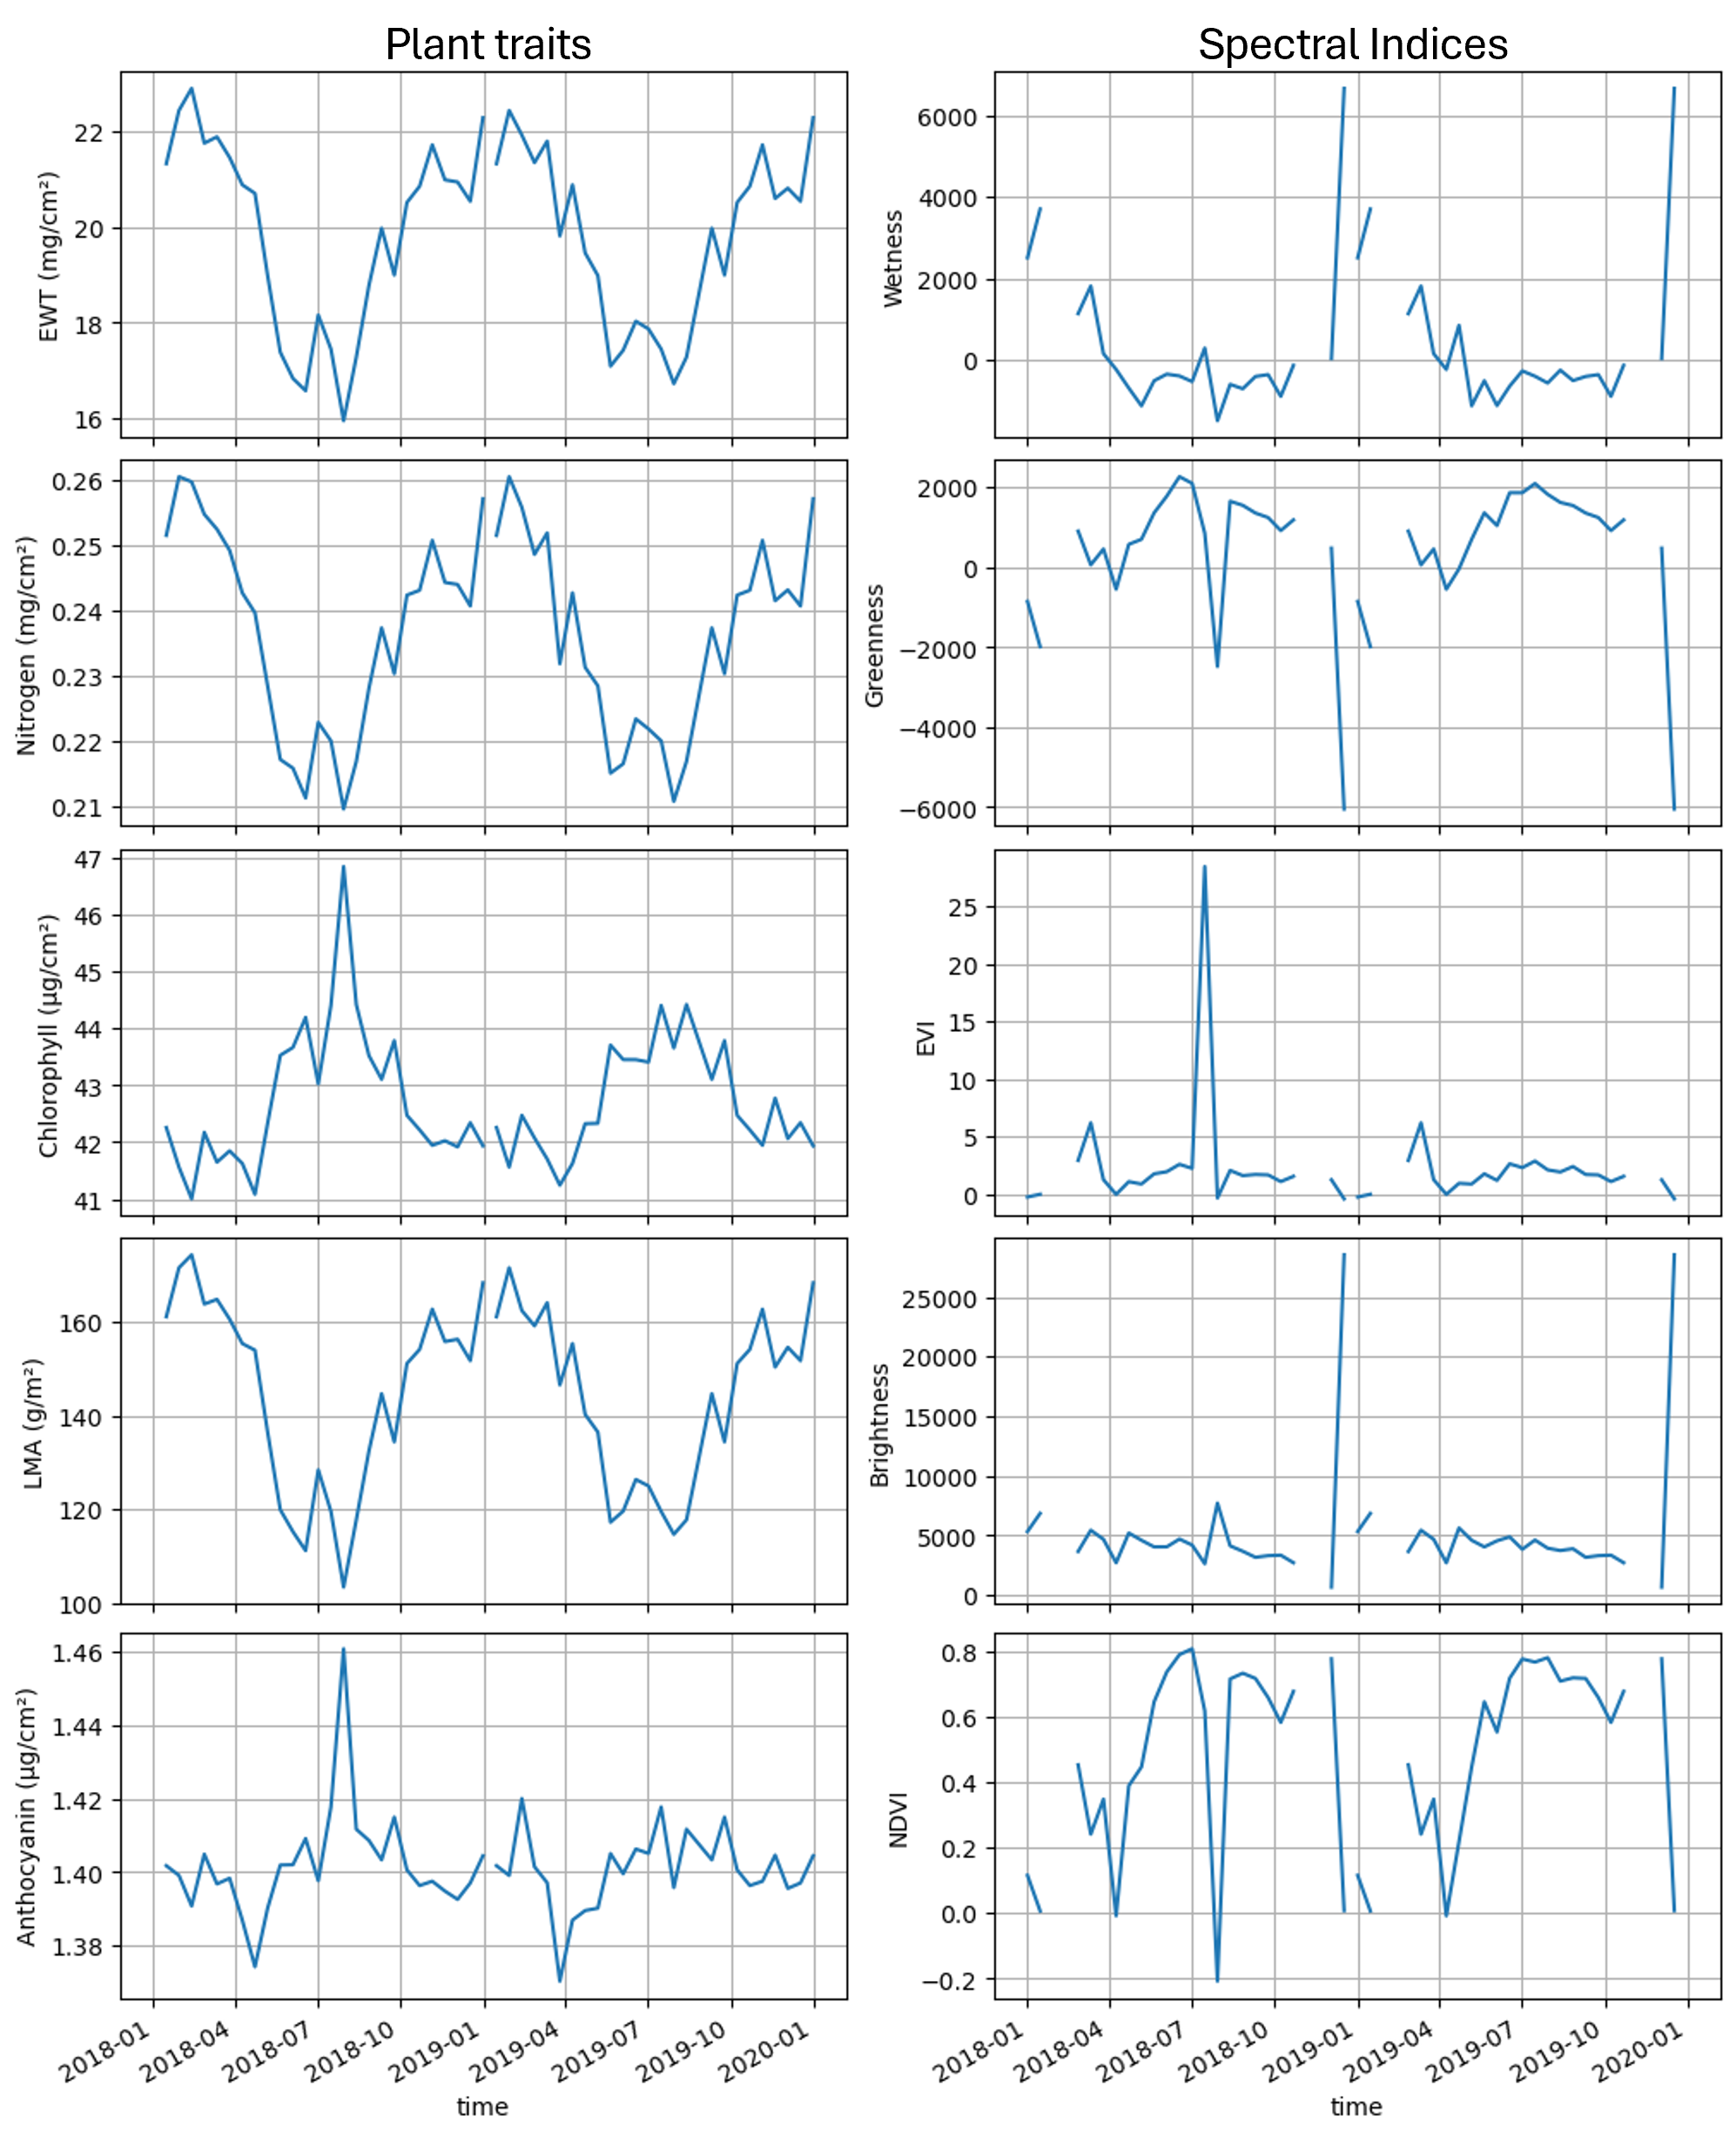
\includegraphics[width=0.8\textwidth]{figures/fig3.png}
%\caption{Comparison between hyperspectral-derived vegetation traits (left) and spectral indices from original Sentinel-2 reflectance (right) for a forest pixel (2018–2019). Trait time series (e.g., EWT, nitrogen, chlorophyll) show smooth, continuous dynamics, whereas spectral indices (e.g., NDVI, EVI, wetness) display discontinuities due to data gaps and sensitivity to non-vegetation factors. The trait cube provides physiologically meaningful information, enhancing the interpretability of vegetation responses beyond traditional indices..}
%\label{fig3}
%\end{figure}

%This comparison underscores the added value of trait-based monitoring in ecological applications. Trait combinations can help distinguish between different types of stress responses—for instance, separating drought-induced senescence from nutrient limitation or photoinhibition. Such specificity is difficult to achieve using broadband indices alone. By enabling the identification of physiological shifts that often precede visible canopy decline, hyperspectral trait data cubes support more reliable early warning, stress attribution, and process-level analysis under global change scenarios \citep{moreno2021early}.


%\subsection*{Example 2: Temporal Dynamics of Plant Water Status and Phenology}

%The plant water content trait derived from hyperspectral data can serve as a proxy for internal water status, which in turn relates to root activity, hydraulic architecture, and drought resilience. By tracking changes in traits such as leaf water content or equivalent water thickness (EWT) over time, it becomes possible to infer belowground functional status indirectly, including root-soil interactions and drought responses \citep{cleverly2013drought}.

%Moreover, temporal shifts in traits such as leaf nitrogen, chlorophyll, or structural properties reflect key phenological transitions (e.g., leaf emergence, senescence) at finer resolutions than phenocam or NDVI-based approaches, providing new insights into intra-annual ecological dynamics.

%\subsection{Example 3: From Plant Functional Types to Trait-Based Dynamic Global Vegetation Models (DGVMs)}

%Current dynamic global vegetation models (DGVMs) often rely on categorical land cover maps or generalised plant functional types, which constrain ecological realism. Species-level mapping is infeasible at large scales, but trait-based representations offer a promising alternative. Trait cubes can provide temporally resolved inputs of SLA, leaf nitrogen, and other physiological properties, allowing for dynamic representation of functional types based on actual plant function rather than fixed categories. This shift could help reconcile model–data mismatches and improve predictions of vegetation–climate feedbacks.

%\subsection{Example 4: Trait-Based Functional Diversity Assessment at Large Scales}

%Current large-scale assessments of functional diversity using airborne or satellite hyperspectral data often rely on proxies such as spectral variance or vegetation indices. Jetz et al. (2016) and Schneider et al. (2017) demonstrated how hyperspectral data from APEX can be used to approximate ecosystem functional diversity using spectral metrics. However, these methods are limited in capturing seasonal trait dynamics.

%Recent advances, such as those presented in Mederer et al. (in review), demonstrate the value of temporally resolved trait cubes for quantifying functional diversity across biomes. Their trait-based products capture both mean trait states and intra-seasonal variability, allowing for more ecologically meaningful comparisons across space and time. Such developments provide a foundation for incorporating continuous, functionally relevant plant traits into biodiversity monitoring and biogeographic analyses.

%\subsection{Example 5: Trait Diversity as a Proxy for Genetic Diversity}
%genetic diversity
%Plant traits derived from hyperspectral data can serve as functional proxies for genetic diversity, particularly when these traits reflect phenotypic variation regulated by heritable genetic factors \citep{Violle2007, Funk2017, Zhao2021}. Many plant traits observable via hyperspectral sensors—such as chlorophyll content, leaf mass per area (LMA), and pigment composition—exhibit intraspecific variation shaped by the interactions of genotypes with their environment \citep{Asner2015, Schweiger2018}. Genetic diversity—defined as genomic variation within and between populations—is a foundation of phenotypic plasticity, adaptive potential, and ecosystem resilience \citep{Barrett2008, Jump2009}. In forest ecosystems, where long-lived species dominate and shape community structure, genetic variation underpins environmentally contingent variation in growth, phenology, and stress tolerance \citep{Petit2006, Alfaro2014}. While molecular methods remain the gold standard for assessing genetic diversity, remotely sensed trait diversity offers a scalable and ecologically meaningful proxy. It has been shown to correlate with genetic structure in some systems and holds promise for scaling genetic information to the landscape level (recently reviewed in \cite{cavender2025spectral}. Moreover, phenotypic variability observed across populations—such as trait differences under drought or nutrient stress—can reflect genotype–environment interactions and local adaptation, and enable analyses of the resistance and resilience of communities to stress \citep{Shakoor2017, Bai2023}. Global policy frameworks increasingly recognise trait diversity and population-level indicators as useful surrogates for monitoring genetic diversity, particularly in large-scale or data-limited contexts \citep{Hoban2020, Hoban2024}.


%\subsection{Example 6: Linking Traits to Carbon and Energy Fluxes}

%Traits derived from hyperspectral data have direct physiological relevance to ecosystem carbon dynamics. For example, leaf nitrogen and chlorophyll content are closely tied to photosynthetic capacity, while leaf mass per area (LMA) relates to respiration and turnover rates \citep{wright2004leaf}. The temporal evolution of these traits can be coupled with flux tower observations to model gross primary productivity (GPP), respiration, and evapotranspiration across space and time \citep{serbin2015remotely}.

%Trait data cubes thus hold the potential to serve as inputs or constraints for carbon flux modeling frameworks, bridging the gap between remote sensing observations and terrestrial ecosystem models.

%\subsection{small summary}

%The transition from multispectral vegetation indices to hyperspectral-derived plant trait data cubes represents a significant advance in ecological remote sensing. These data products enable a shift from empirical greenness proxies to mechanistic, trait-based characterisations of vegetation function. The examples presented above demonstrate the diverse applications of trait cubes across spatial and ecological scales: (1) at local to regional scales, trait cubes enable high-frequency monitoring of vegetation physiological status (Examples 1, 2, and 6), including plant condition, water status, phenological development, and ecosystem carbon and energy fluxes; (2) at landscape to biome scales, they support assessments of functional and genetic diversity (Examples 4 and 5) by capturing intra- and interspecific trait variation across environmental gradients and time; and (3) at the global modeling scale, trait cubes provide continuous, ecologically meaningful parameters to replace categorical land cover or PFT representations in dynamic global vegetation models (Example 3). Together, these examples underscore the integrative value of hyperspectral trait data cubes in ecological monitoring, biodiversity assessment, and Earth system modelling, and highlight their potential for improving our understanding of ecosystem dynamics under global environmental change.


%\section{Target 2: Explore the full potential of hyperspectral data} \label{sec3}

%As plant trait time series become increasingly accessible through hyperspectral–multispectral fusion, their integration into ecological analysis opens new avenues beyond traditional vegetation indices based on multispectral data. These trait-based data cubes—comprising key variables such as chlorophyll content, leaf mass per area (LMA), equivalent water thickness (EWT), and leaf area index (LAI)—offer high-resolution, biochemically grounded information that supports a more mechanistic understanding of ecosystem function and resilience. In this section, we outline three major pathways through which these hyperspectral-derived trait cubes can support ecosystem monitoring: (1) integration with complementary data sources to enrich existing monitoring products; (2) support for ecological and Earth system model development; and (3) enhanced global change research through trait-based indicators.




%\subsection{Enriching Earth system models via traits data cube}\label{subsec1}
%\cite{scheffer2009early,boulton2022pronounced,tai2023linking}. These insights are vital for designing effective mitigation and adaptation strategies in the Anthropocene. Ecosystem process models such as LPJ and Biome-BGC represent vegetation at large scales using fixed plant functional types (PFTs), each assigned with mean trait values. This approach oversimplifies functional diversity and ignores intra- and inter-annual variation in key traits such as nitrogen concentration, LAI, or non-structural carbohydrates (NSC) \cite{verrelst2019quantifying,mederer2025plant}. Land surface properties are also assumed to be temporally stable over simulation intervals, which limits model responsiveness to droughts, land-use changes, or disturbance events. Incorporating time-series trait data into DGVMs enables the transition from coarse PFT-based parameterizations to trait-based dynamic modeling. This improves the physiological realism of carbon and water flux simulations and increases predictive skill under extreme climate events or changing vegetation regimes. For example, real-time NSC and EWT dynamics can inform ecosystem vulnerability and carbon allocation strategies under stress.

%\subsection{Enriching Earth system models via traits data cube}\label{subsec1}
%This trait-based lens is particularly important for understanding and predicting the stability of terrestrial carbon sinks \cite{xu2021trait}. Accurate trait data can inform assessments of photosynthetic capacity, water-use efficiency, and stress responses—critical for modelling carbon sequestration potential and its directionality under climate change \cite{gago2014opportunities}. Integrating trait cubes into Earth system models could therefore improve forecasts of terrestrial carbon fluxes by linking biological processes with climate variability and disturbance regimes \cite{anderegg2015tree,peng2021global}. Additionally, trait data can reveal spatial patterns of vegetation adaptation and maladaptation, offering early-warning signals of biome shifts, forest dieback, or ecosystem transitions that traditional land cover maps may miss 
% SIF
% environmental DNA, below ground diversity?
%Integrating hyperspectral remote sensing with other Earth observation and \textit{in situ} measurements is essential for advancing ecological monitoring, improving trait estimation, and supporting model validation. Hyperspectral sensors provide detailed spectral information linked to plant biochemical and physiological traits, but their effectiveness increases when combined with complementary data sources that capture structural and functional ecosystem properties. For example, coupling hyperspectral data with canopy structure from LiDAR or SAR improves trait characterisation in vertically complex forests. Likewise, integrating hyperspectral and thermal data enables more accurate detection of plant stress and assessments of functional diversity under climate extremes. It further offers the opportunity to identify the actual stressor through investigating the degradation of specific traits such as leaf water content, pigments or nitrogen status. Such multi-source datasets enhance the robustness of trait retrievals and serve as intermediate validation layers. Validation is the bottleneck when ensuring the reliability of hyperspectral products \citep{cherif2023spectra,mederer2025plant}, and \textit{in situ} observations, such as those from eddy covariance systems, provide essential flux data for calibration and evaluation. The FLUXNET network, with over 140 globally distributed sites across diverse biomes, offers standardised, high-quality localised remote sensing measurements that anchor remote observations and inform ecosystem models. Together, these integrated approaches establish a robust framework for generating and validating remote sensing products in ecological research.




%\subsection{Supporting the Development of Ecological and Earth System Models}\label{subsec3}

%Ecological and Earth system models are critical for predicting carbon dynamics, vegetation-climate interactions, and ecosystem responses to disturbance. However, a major limitation across model classes lies in their reliance on static, generalised plant trait inputs and infrequent land surface updates. These assumptions fail to represent transient ecosystem states and trait plasticity, leading to considerable uncertainty under changing environmental conditions (and links to genotype-by-environment interactions). Integrating trait cubes—biweekly, spatially continuous time series of plant functional traits derived from hyperspectral observations—offers a new path toward improving model structure, parameterisation, and scaling.



% + radiative transfer models
%Radiative transfer models (RTMs) such as PROSAIL \cite{jacquemoud2009prospect+} and DART \cite{gastellu2004dart} provide a physically grounded framework to simulate trait values from canopy reflectance. Integrating time series or plant traits retrieved from hyperspectral data enhances the realism of RTM inversions, improving alignment with seasonal and phenological dynamics \cite{verrelst2019quantifying,mederer2025plant}. However, most RTMs oversimplify real-world vegetation by assuming fixed canopy structures, homogeneous leaf distributions, and static physiology. As a result, they often fail to reproduce observed spectra in heterogeneous or stress-responsive ecosystems (ill-posed problem) \cite{kattenborn2019radiative,ali2021machine}. Despite these limitations, RTMs remain valuable—particularly in data-scarce regions and as physical priors in hybrid modeling approaches. Embedding RTMs into neural networks as differentiable components allows models to retain physical interpretability while adapting to observational data \cite{sun5107112bridging,she2024spectra}. Transfer learning extends their utility by using RTM simulations for pre-training, followed by fine-tuning on field data \cite{zhang2021domain}. Together, these strategies bridge physical modelling and data-driven learning, improving generalisation and trait estimation in diverse ecosystems.


% Individual-Based and Gap Models
%Individual-based models (IBMs) such as FORMIND \cite{kohler1998effects} and FORMIX3 \cite{huth1998rain} explicitly simulate forest structure, competition, and succession by modeling trees as discrete units. These models capture stand dynamics well but typically rely on static or coarsely aggregated trait inputs (e.g., fixed leaf mass per area or chlorophyll content), and land cover inputs are updated annually or remain fixed. As a result, IBMs struggle to represent seasonal transitions, physiological responses, or disturbance legacies, reducing their accuracy in simulating mortality, recruitment, and biomass turnover. Traits cubes derived from hyperspectral time series enable the introduction of spatially and temporally dynamic trait inputs—such as seasonal variation in chlorophyll, EWT, or LMA—thereby improving predictions of individual tree growth, stress response, and regeneration. This supports better representation of competitive interactions, phenological synchrony, and stand-scale heterogeneity.

% Dynamic Global Vegetation Models (DGVMs)
%Ecosystem process models such as LPJ and Biome-BGC represent vegetation at large scales using fixed plant functional types (PFTs), each assigned with mean trait values. This approach oversimplifies functional diversity and ignores intra- and inter-annual variation in key traits such as nitrogen concentration, LAI, or non-structural carbohydrates (NSC) \cite{verrelst2019quantifying,mederer2025plant}. Land surface properties are also assumed to be temporally stable over simulation intervals, which limits model responsiveness to droughts, land-use changes, or disturbance events. Incorporating time-series trait data into DGVMs enables the transition from coarse PFT-based parameterizations to trait-based dynamic modeling. This improves the physiological realism of carbon and water flux simulations and increases predictive skill under extreme climate events or changing vegetation regimes. For example, real-time NSC and EWT dynamics can inform ecosystem vulnerability and carbon allocation strategies under stress.

% Eco-Physiological Submodels
%Many ecosystem models contain embedded physiological components such as the Farquhar photosynthesis model or the Ball–Berry stomatal conductance model, which require accurate inputs of traits including Vcmax, Jmax, chlorophyll content, and LMA \cite{sun5107112bridging,ali2021machine}. However, in practice, these submodels are typically run with trait values that are either constant or calibrated under limited conditions, failing to reflect phenological shifts or physiological acclimation. By providing frequent, spatially resolved trait updates, traits cubes enhance the mechanistic representation of photosynthetic efficiency, light-use dynamics, and stress physiology. %Integrating seasonally varying chlorophyll and LMA directly informs models of GPP and respiration, while time-varying NSC and EWT support estimation of drought-induced mortality risk. Embedding these trait updates improves the fidelity of ecosystem carbon cycle predictions, especially under transient or disturbed conditions.



%\subsection{Enhancing Global Change Research with Trait Cubes}\label{subsec4}
%Despite progress in Earth observation and ecosystem modeling, significant limitations remain in understanding vegetation responses to global change across spatial scales \cite{higgins2023shifts}. Most global vegetation products—particularly those derived from climate-driven dynamic global vegetation models (DGVMs) or coarse-resolution satellite data—are simplified representations that fail to capture plant functional diversity and physiological traits at fine spatial and temporal scales. Downscaled datasets often rely heavily on climate variables and land cover classifications, introducing structural uncertainty and masking sub-grid ecological heterogeneity. In contrast, hyperspectral trait cubes provide rich, high-resolution spatiotemporal data on ecophysiological traits, such as chlorophyll content, LMA, or equivalent water thickness, offering new opportunities to monitor ecosystem changes with greater specificity and accuracy \cite{zhao2021hyperspectral}. These data can help reduce uncertainty in ecosystem assessments by grounding predictions in empirically observable traits rather than generalized proxies or model assumptions.

%Plant traits offer a mechanistic link between organisms and their environment, representing functional strategies for survival, growth, and resource use under changing conditions \cite{solbrig1994plant,funk2017revisiting}. Incorporating trait-based data into global change research thus enhances the capacity to assess not only what is changing but how and why it changes \cite{xu2021trait,green2022trait}. Trait cubes allow for continuous tracking of functional diversity and vegetation health across time and space, enabling a shift from static land cover maps to dynamic, physiology-informed monitoring. Moreover, such data enable trait-based indicators of ecosystem vulnerability, resilience, and tipping points—key aspects often missed in purely spectral or structural products \cite{gallagher2021guide,brown2023trait}.






\section{Challenges and opportunities}\label{subsec2}
Achieving these targets requires integrating traditional methods with emerging technologies, interdisciplinary collaboration, and open science initiatives.

% challenges--
% uncertainty
Key challenges in integrating hyperspectral data into ecological monitoring include overcoming data availability and temporal coverage constraints, computational and technical hurdles, and fostering interdisciplinary collaboration. Despite the promise of more spaceborne hyperspectral sensors, such as CHIME and SBG in the coming decade, current sensors like EnMAP and PRISMA offer limited spatial and temporal coverage. Although future missions may expand coverage, they cannot address the lack of historical data, necessitating the reconstruction of past data using other sources—an approach that inherently introduces uncertainty. Furthermore, maintaining consistency in techniques and sensor settings during ecosystem monitoring is essential to ensure robust long-term statistical analyses. This requirement must be carefully balanced with integrating new technologies.

% computational and expert knowledge required
The computational and technical complexities of hyperspectral data processing are also substantial. For instance, even a modest study area of 30 km by 30 km, sampled bi-weekly over a decade, can result in XX terabytes of data, posing storage, processing, and analysis challenges. Additionally, effective use of hyperspectral data demands not only advanced machine learning models for data fusion (e.g., hyperspectral, multispectral, LiDAR, SAR) but also scientists with cross-disciplinary expertise who can fully leverage the strengths of each data source. 

% the constantly asked question: extensive data
For hyperspectral data, the large volume of information remains a persistent challenge. One major limitation is the constrained satellite-to-ground data downlink capacity, which complicates data acquisition. To address this, missions such as EnMAP and PRISMA adopt a task-based acquisition strategy. When a specific area is targeted for observation, neighbouring regions are often deprioritised or omitted entirely, resulting in incomplete data coverage. To mitigate these limitations, edge computing has gained significant attention over the past decade. This approach is particularly favoured by small commercial hyperspectral satellite missions, as it allows for onboard data processing, reducing the need for extensive downlink and enabling more efficient use of limited transmission bandwidth. For ecological applications, it is recommended that users directly utilise plant trait products derived from hyperspectral data, such as the example presented in Section \ref{sec2}, or apply simplified computational models to process long-term hyperspectral datasets. As data volumes continue to grow and machine learning models evolve rapidly, technological advancements are expected to further alleviate the challenges associated with hyperspectral data acquisition and processing.


% call for scientist
Here, we make a call to action for researchers and policymakers. Effective cross-disciplinary collaboration is essential for bridging the gaps between remote sensing and ecology, ensuring a seamless connection between data producers and end-users, and fostering a positive feedback loop that enhances data product quality. To fully realise the potential of global hyperspectral data applications, it is crucial to promote the scalable collection and integration of hyperspectral data from field, UAV, and airborne platforms. These datasets should be openly shared and adhere to standardised protocols, ideally established by leading laboratories, to ensure consistent data pre-processing and sharing practices. Policymakers who understand the capabilities of hyperspectral data—particularly its ability to detect detailed ecological traits—will be better equipped to support its integration into ecosystem monitoring and conservation strategies. Such awareness can accelerate the adoption of hyperspectral technology, driving more effective ecological management and climate resilience efforts.

The feasibility of long-term backcasting depends on the spectral richness and radiometric stability of the multispectral archive. Sentinel-2 provides comparatively rich spectral information that supports trait modelling. Extending trait backcasting further in time using Landsat data may be feasible for selected structural or pigment-related traits, but is likely to be limited for biochemically complex traits due to reduced spectral resolution. The achievable temporal depth therefore depends on the trait of interest and the spectral characteristics of the multispectral sensor.



\section{Conclusion}\label{subsec5}

Hyperspectral data enable the quantification of plant and canopy biochemical traits, offering unprecedented insights into ecosystem function. In this paper, we introduce the concept of constructing time series of hyperspectral-derived plant traits already at present, despite limitations on available time series, by leveraging time series of multispectral data. This approach addresses the current limitations in observation frequency that hinder the application of hyperspectral data in real-world ecosystem analyses. We highlight the value of hyperspectral data not only as a standalone resource but also as a complementary input to other datasets, physical models, and biological systems monitoring, enhancing the accuracy and scope of ecological assessments. While we discuss associated challenges—such as data volumes, downlink constraints, interpretability, and processing complexity—we also emphasise emerging opportunities, including edge computing and simplified trait-based analysis approaches. Realising the full potential of hyperspectral remote sensing requires a coordinated global effort to establish priorities and synthesise evidence, including through ecological monitoring networks, open data sharing, and transdisciplinary collaboration among ecologists, remote sensing scientists, data analysts, and policymakers. Looking ahead, we join the call to the ecological community to proactively adopt these advanced technologies to address critical challenges in ecosystem analysis, particularly under accelerating climate change \cite{cavender2025spectral}. Such advancements have the potential to directly inform global ecological governance, providing essential data for conservation planning and evidence-based policy-making.

%%%%%%%%%%%%%%%%%%%%%%%%%%%%%%%


\bmhead{Supplementary information}

If your article has accompanying supplementary file/s please state so here. 

Authors reporting data from electrophoretic gels and blots should supply the full unprocessed scans for key as part of their Supplementary information. This may be requested by the editorial team/s if it is missing.

Please refer to Journal-level guidance for any specific requirements.

\bmhead{Acknowledgements}

We thank Maximilian Soechting for his professional input and constructive suggestions that contributed to the development of Figure 2.

\section*{Declarations}

Some journals require declarations to be submitted in a standardised format. Please check the Instructions for Authors of the journal to which you are submitting to see if you need to complete this section. If yes, your manuscript must contain the following sections under the heading `Declarations':

\begin{itemize}
\item Funding


We want to thank the editors and anonymous reviewers for their constructive comments that helped to improve the manuscript. The authors acknowledge the support from the German Federal Ministry for Economic Affairs and Climate Action (BMWK) and the German Aerospace Center (DLR) for the project "TEE Cube - Time-varying AI-based Mapping of Ecosystem Conditions and Extents Using Multi-source Earth Observation Data Cubes".

\item Conflict of interest/Competing interests (check journal-specific guidelines for which heading to use)
\item Ethics approval and consent to participate
\item Consent for publication
\item Data availability 

The authors acknowledge the German Aerospace Center (DLR) for sharing airborne flight campaign data.


\item Materials availability
\item Code availability 
\item Author contribution
\end{itemize}

\noindent


\begin{appendices}
\section{}\label{secA1}
\end{appendices}


\bibliography{bibliography}% common bib file
%% if required, the content of .bbl file can be included here once bbl is generated
%%\input sn-article.bbl

\end{document}
